\chapter{Modelo Matemático} \label{ch:mathematical_model}

Segundo \citeonline{bib:maliska}, a solução numérica de qualquer problema físico requer a sua prévia modelagem matemática. Um modelo matemático é uma representação de um sistema real através de equações. Essas equações são obtidas ao se fazerem hipóteses sobre o comportamento do sistema estudado, e a representatividade do modelo depende das simplificações feitas nesse processo.

Este capítulo aborda os aspectos matemáticos pertinentes ao Método dos Elementos Discretos. São abordados os principais conceitos referentes aos sistemas de partículas, e apresentadas as equações de movimento que governam o problema. Por fim, é apresentado o algoritmo de Gear, responsável por resolver as equações.

\section{Sistemas de Partículas}

As partículas são os elementos fundamentais do Método de Elementos Discretos. De acordo com a definição apresentada por \citeonline{bib:sampaio}, partículas são consideradas corpos rígidos. Por serem indeformáveis, fica implícita a hipótese de que não ocorrem deformações plásticas nesses elementos, e então eles preservam a sua geometria mesmo após colisões.

A princípio, o DEM suporta geometrias arbitrárias para seus elementos. Entretanto, devido a limitações de modelos físicos e de avaliação das colisões, em geral consideram-se formatos básicos como esferas, superelipsoides e poliedros. Geometrias mais complexas podem ser geradas pela associação de geometrias mais simples em partículas compostas \cite{bib:sampaio,bib:computational_granular_dynamics}.

Um sistema de partículas é, por sua vez, um conjunto de partículas que interagem entre si. Considera-se que o sistema possua um referencial global fixo, a partir do qual as demais grandezas vetoriais são definidas.

A cada partícula está associada uma função posição que determina, vetorialmente, a posição de seu centro de massa com relação à origem do sistema. A orientação de um elemento é a orientação do seu sistema de eixos local com relação ao sistema global. Com isso, cada partícula possui seis graus de liberdade: três translações e três rotações \cite{bib:sampaio}. Os elementos discretos ainda contêm diversas \textit{propriedades}, as quais são determinantes para as suas interações.

As translações e rotações das partículas são determinadas através da solução das equações de movimento, detalhadas na seção \ref{sec:equations_of_motion}. Essas equações dependem das interações que ocorrem entre as partículas. Em um sistema qualquer, essas interações podem ser de diversas naturezas, tais quais colisões mecânicas, troca de cargas elétricas, transferência de calor, e outras. No entanto o DEM considera, a princípio, apenas as colisões.

\section{Equações de Movimento} \label{sec:equations_of_motion}

Na dinâmica de partículas, os elementos estudados são considerados corpos rígidos, aos quais se aplicam as leis de Euler para o movimento \cite{bib:sampaio, bib:dynamics_of_multibody_systems}.

Em um sistema inercial fixo, considera-se uma partícula de massa \(\mass\) com um centro de massa cuja posição é descrita pela função vetorial \(\position\). Além disso, considera-se que a partícula possua uma velocidade angular \(\angularVelocity\) e um tensor momento de inércia \(\tensorOfInertia\) definido com relação ao seu centro de massa.

Conforme demonstrado por \citeonline{bib:dynamics_of_multibody_systems}, o \textit{momento linear} e o \textit{momento angular} da partícula, denotados respectivamente por \(\linearMomentum\) e \(\angularMomentum\), são então dados por
\begin{gather*}
	\linearMomentum = \mass\cdot\velocity, \\
	\angularMomentum = \position\cross\linearMomentum + \tensorOfInertia\cdot\angularVelocity.
\end{gather*}

\subsection{Primeira Lei de Euler}

A primeira lei de Euler trata do movimento de translação. Ela se expressa através da equação
\begin{equation} \label{eq:euler_first}
	\resultingForce = \deriv{1}{\linearMomentum},
\end{equation}
sendo \(\resultingForce\) o vetor força resultante sobre a partícula. Para o caso em que a massa do corpo é constante, a primeira lei de Euler torna-se equivalente à segunda lei de Newton:
\begin{equation} \label{eq:motion_first}
	\resultingForce = \mass\cdot\acceleration.
\end{equation}

A equação \eqref{eq:euler_first} é aplicada para os fenômenos de fragmentação e aglutinação, casos em que partículas são divididas ou unidas, sendo que a massa de cada partícula isoladamente não é constante. \citeonline{bib:computational_granular_dynamics} apresenta métodos que descrevem o fenômeno de fragmentação. Tais situações, porém, são tratadas separadamente, de modo que a equação \eqref{eq:motion_first} é a que se considera para o estudo da evolução do sistema.

De acordo com o princípio da superposição, a força resultante sobre a partícula é igual à soma vetorial todas as forças aplicadas sobre ela. Essas forças são comumente divididas em \textit{forças internas} e \textit{forças externas} ao sistema. As forças internas são aquelas oriundas das interações entre os elementos do sistema, enquanto as forças externas são atribuídas a elementos exteriores.

Para a translação, os movimentos ocorrem separadamente em cada eixo coordenado de modo que os algoritmos de solução da equação \eqref{eq:motion_first} são facilmente generalizados de duas para três dimensões. Ainda, cabe observar que a primeira lei de Euler independe da posição do eixo de referência.

\subsection{Segunda Lei de Euler}

A segunda lei de Euler, por sua vez, é o análogo rotacional da primeira:
\begin{equation*} % \label{eq:euler_second}
	\resultingTorque = \deriv{1}{\angularMomentum},
\end{equation*}
em que \(\resultingTorque\) é o torque resultante sobre a partícula calculado com relação ao seu centro de massa. Para partículas com massa constante, é possível obter
\begin{equation} \label{eq:motion_second}
	\resultingTorque = \deriv{1}{\angularMomentum} = \tensorOfInertia\cdot\deriv{1}{\angularVelocity} + \angularVelocity\cross\pqty{\tensorOfInertia\cdot\angularVelocity}.
\end{equation}

Novamente, a hipótese de que a massa da partícula é constante é geralmente considerada. 

Entretanto, mesmo diante de situações em que \(m\) é constante, a resolução da equação \eqref{eq:motion_second} possui algumas complicações em simulações tridimensionais. Isso se deve ao fato de que são necessárias parametrizações para a orientação da partícula, e não ocorre que a velocidade angular seja a derivada desses parâmetros. Só é possível escrever \(\angularVelocity = \deriv{1}{\orientation}\) quando a direção da rotação é constante \cite[p. 32]{bib:dynamics_of_multibody_systems}.

A cada corpo estão associados \textit{eixos principais}, formados pelos autovetores da matriz de momento de inércia \(\matrixOfInertia\). Ao se utilizarem como sistema de referência os eixos principais, a matriz de inércia assume forma diagonal:
\begin{equation*}
	\matrixOfInertia =
	\begin{pmatrix}
		\momentOfInertia_1 & 0 & 0 \\
		0 & \momentOfInertia_2 & 0 \\
		0 & 0 & \momentOfInertia_3 \\
	\end{pmatrix},
\end{equation*}
e, reescrevendo, nessas coordenadas, o torque resultante como \(\explicitVectorCoordinates{\torqueScalar}\), a velocidade angular como \(\explicitVectorCoordinates{\angularVelocityScalar}\) e a aceleração angular como \(\explicitVectorCoordinates{\deriv{1}{\angularVelocityScalar}}\), a equação \eqref{eq:motion_second} se transforma no sistema de equações
\begin{equation} \label{eq:motion_second_system}
	\left\lbrace
	\begin{array}{l}
		\momentOfInertia_1\deriv{1}{\angularVelocityScalar}_1 - \pqty{\momentOfInertia_2 - \momentOfInertia_3}\angularVelocityScalar_2\angularVelocityScalar_3 = \torqueScalar_1 \\
		\momentOfInertia_2\deriv{1}{\angularVelocityScalar}_2 - \pqty{\momentOfInertia_3 - \momentOfInertia_1}\angularVelocityScalar_3\angularVelocityScalar_1 = \torqueScalar_2 \\
		\momentOfInertia_3\deriv{1}{\angularVelocityScalar}_3 - \pqty{\momentOfInertia_1 - \momentOfInertia_2}\angularVelocityScalar_1\angularVelocityScalar_2 = \torqueScalar_3
	\end{array}
	\right.
	.
\end{equation}

Esse sistema pode ser resolvido de forma análoga à primeira lei de Euler, conforme discutido na \autoref{eq:motion_equations_solution}. Os valores de \(\momentOfInertia_1\), \(\momentOfInertia_2\) e \(\momentOfInertia_3\) são dependentes da geometria da partícula e da distribuição de massa no seu interior. Em geral, essas características já são conhecidas no início das simulações.

Entretanto o sistema \eqref{eq:motion_second_system} exige que se conheçam os eixos principais da partícula, isto é, sua orientação. Esses eixos, porém, movem-se e rotacionam junto com o corpo, e então são variantes no tempo. Para se resolver o problema no caso geral, são propostas parametrizações, tais quais os ângulos de Euler, os ângulos de Bryan, e os parâmetros de Euler-Rodrigues \cite{bib:dynamics_of_multibody_systems}. Mais detalhes sobre essas parametrizações são encontrados no \autoref{app:three_dimensional_rotation}.

\alert{Verificar que os detalhes foram explicados no apêndice}

Duas simplificações que podem se aplicar à equação \eqref{eq:motion_second} são: que a direção das rotações é sempre constante; ou que as partículas são esféricas. No primeiro caso, o sistema se torna equivalente a um problema bidimensional. Essa situação é tratada na \autoref{subsubsec:constant_rotation}. Já no segundo caso, como explicado na \autoref{subsubsec:rotation_of_spherical_particles}, qualquer sistema de eixos centrado no centro de massa da partícula é um sistema de eixos principais, e então a orientação das partículas não é mais necessária para a determinação de \eqref{eq:motion_second_system}.

O caso geral de rotações em três dimensões é apresentado no \autoref{app:three_dimensional_rotation}.

\subsubsection{Direção de Rotação Constante} \label{subsubsec:constant_rotation}

Para rotações com direção constante, é possível definir um vetor \(\angularVelocityVersor\) constante e unitário tal que a velocidade angular da partícula se escreve como
\[
	\angularVelocity = \angularVelocityScalar\cdot\angularVelocityVersor,
\]
sendo \(\angularVelocityScalar\) uma função escalar do tempo. Já que a velocidade angular é diferenciável, \(\angularVelocityScalar\) é contínua e, portanto, integrável, do que é possível escrever
\begin{gather*}
	\angularVelocityScalar = \deriv{1}{\orientationScalar}, \\
	\angularVelocity = \deriv{1}{\orientationScalar}\cdot\angularVelocityVersor, \text{e} \\
	\angularAcceleration = \deriv{2}{\orientationScalar}\cdot\angularVelocityVersor.
\end{gather*}

Nesse caso, \(\orientationScalar\) é uma função que representa o ângulo de rotação que a partícula faz com uma orientação de referência, como representado na figura \ref{fig:particle_scalar_orientation}.

\begin{figure}[h]
	\caption{Ângulo de rotação de uma partícula com relação à posição de referência em simulações com direção de rotação constante}
	% \vspace{-0.5cm}
	\begin{center}
		\alert{Colocar imagem representando a orientação de uma partícula em rotações com direção constante}
		% 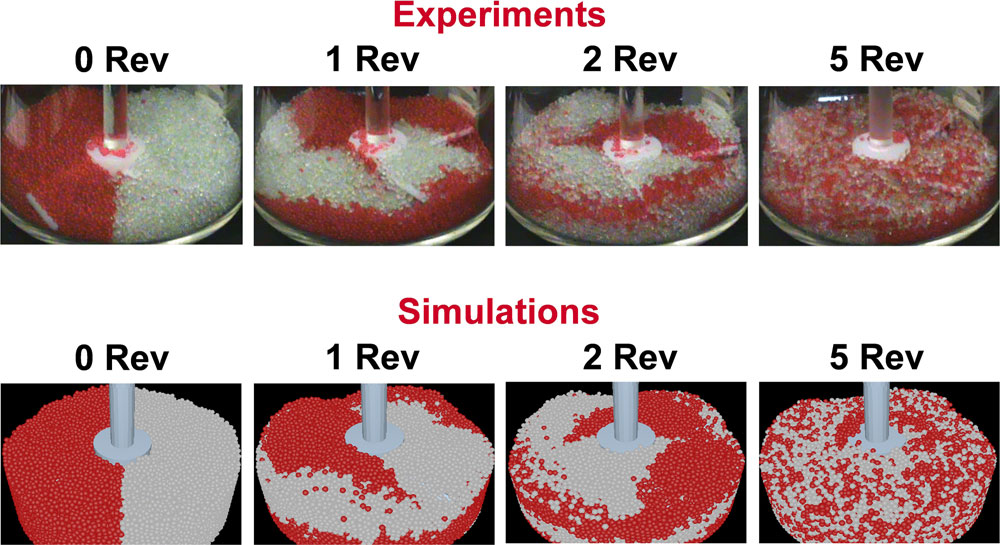
\includegraphics[width=0.65\textwidth]{images/drug_production.png}
	\end{center}
	% {\centerline{\includegraphics[scale=#2]{#1}}}
	% \vspace{-0.2cm}
	\label{fig:particle_scalar_orientation}
	\legend{Fonte: \alert{Citar fonte}.}
	% \vspace{-1cm}
\end{figure}

Com isso, a equação \eqref{eq:motion_second} fica
\begin{equation*}
	\resultingTorque = \deriv{2}{\orientationScalar}\cdot\pqty{\tensorOfInertia\cdot\angularVelocityVersor}
		+ \deriv{1}{\orientationScalar}^2\cdot\pqty{\angularVelocityVersor\cross\tensorOfInertia\cdot\angularVelocityVersor}
\end{equation*}

\alert{Arrumar o caso anterior. Supor que as rotações são em torno do eixo \zAxis}

\alert{Terminar}

\subsubsection{Rotação de Partículas Esféricas} \label{subsubsec:rotation_of_spherical_particles}

\alert{Escrever}

\subsection{Solução das Equações de Movimento} \label{eq:motion_equations_solution}

Para a determinação do comportamento do sistema, é necessária a obtenção das soluções para as equações \eqref{eq:motion_first} e \eqref{eq:motion_second}.

\alert{E daí?}

\section{Modelos de Força de Colisão} \label{sec:collision_force_models}

Dentre as interações entre partículas do sistema, as mais comumente encontradas são as forças de colisão que surgem durante o contato entre elementos diferentes. Os principais parâmetros considerados para o cálculo das forças de colisão são a geometria das partículas, as suas propriedades físicas, a velocidade relativa no ponto de contato e a \textit{superposição}.

\alert{Explicar melhor isso, principalmente considerando \citeonline{bib:sampaio}}

Os modelos de colisão mais simples são aqueles que ocorrem entre partículas esféricas ou entre uma partícula esférica e uma parede plana.

\alert{Falar do coeficiente de restituição. Um bom exemplo é \citeonline{bib:linear_dashpot_revisited}}

\citeonline{bib:sampaio}

\alert{Terminar}

\section{Extrapolação de Funções}
\label{sec:extrapolation}

Nos métodos numéricos, a extrapolação de funções possui um papel fundamental por permitir a estimativa de valores além do conjunto previamente conhecido.

Para simplificação da notação, dada uma função \(y: X\to Y\), define-se
\[\drvec{\taylorOrder}{y} = \pqty{y, \deriv{1}{y}, \deriv{2}{y}, \dots, \deriv{\taylorOrder}{y}}\]
nos pontos em que todas as coordenadas estiverem definidas.

Conforme demonstrado por \citeonline{bib:extrapolation}, métodos de extrapolação lineares para uma função e suas derivadas podem ser escritos na forma
\[
\begin{pmatrix}
	\predicted{y} \\
	\predicted{\deriv{1}{y}} \\
	\predicted{\deriv{2}{y}} \\
	\vdots \\
	\predicted{\deriv{\taylorOrder-1}{y}} \\
	\predicted{\deriv{\taylorOrder}{y}}
\end{pmatrix}
=
\begin{pmatrix}
	a_{0,0} & a_{0,1} & a_{0,2} &  & a_{0,\taylorOrder-1} & a_{0,\taylorOrder} \\
	a_{1,0} & a_{1,1} & a_{1,2} & \cdots & a_{1,\taylorOrder-1} & a_{1,\taylorOrder} \\
	a_{2,0} & a_{2,1} & a_{2,2} &  & a_{2,\taylorOrder-1} & a_{2,\taylorOrder} \\
     & \vdots & & \ddots & & \vdots \\
    a_{\taylorOrder-1,0} & a_{\taylorOrder-1,1} & a_{\taylorOrder-1,2} &  & a_{\taylorOrder-1,\taylorOrder-1} & a_{\taylorOrder-1,\taylorOrder} \\
    a_{\taylorOrder,0} & a_{\taylorOrder,1} & a_{\taylorOrder,2} & \cdots & a_{\taylorOrder,\taylorOrder-1} & a_{\taylorOrder,\taylorOrder}
\end{pmatrix}
\cdot
\begin{pmatrix}
	y \\
	\deriv{1}{y} \\
	\deriv{2}{y} \\
	\vdots \\
	\deriv{\taylorOrder-1}{y} \\
	\deriv{\taylorOrder}{y}
\end{pmatrix}
\]
ou, de forma mais simples,
\begin{equation}
	\drvec{\taylorOrder}{\predicted{y}} = A \cdot \drvec{\taylorOrder}{y}.
\end{equation}
em que a matriz \(A\) é determinada pelo método escolhido e \(\drvec{\taylorOrder}{\predicted{y}}\) é o vetor de derivadas de \(y\) \textit{predito}.

Dentre os métodos de extrapolação mais utilizados estão o método de expansão de Taylor, o método de Richardson, o método de interpolação de Aitken e os métodos de Runge-Kutta, cada qual com diferentes características em termos de exatidão e estabilidade \cite{bib:gear_book}.

\alert{dizer por que escolhemos o de Taylor}

O método de extrapolação por expansão de Taylor é fundamentado pelo \nameref{theo:taylor}.

\begin{theorem}[Teorema  de Taylor] \label{theo:taylor}
	Seja \(y\) uma função com derivadas \(\deriv{1}{y},\dots,y^{\pqty{\taylorOrder+1}}\) todas definidas em um conjunto que contenha \(\bqty{t, t+\Dt}\), e seja \(R_{\taylorOrder, t, y}\) definida por
    \begin{equation*}
    	y(t + \Dt) = y(t) + \deriv{1}{y}(t)\cdot\Dt + \dots + \dfrac{\deriv{\taylorOrder}{y}(t)}{\taylorOrder!}\cdot\Dt^\taylorOrder + R_{\taylorOrder, t, y}(\Dt).
    \end{equation*}
    Então
    \begin{equation} \label{eq:remainder_limit}
    	\lim_{\Dt \rightarrow 0} \dfrac{R_{\taylorOrder, t, y}(\Dt)}{\Dt^\taylorOrder} = 0.
    \end{equation}
\end{theorem}

Uma versão mais completa desse teorema é apresentada e demonstrada por \citeonline{bib:spivak}.

A função \(R_{\taylorOrder, t, y}\) é o resto de ordem \(\taylorOrder\) para a função \(y\) no entorno de \(t\). A equação \eqref{eq:remainder_limit} indica que o resto é um termo da ordem de \(\Dt^{\taylorOrder+1}\), e motiva a aproximação
\begin{equation} \label{eq:taylor_trunc}
    y(t + \Dt) \approximately y(t) + \deriv{1}{y}(t)\cdot\Dt + \dots + \dfrac{\deriv{\taylorOrder}{y}(t)}{\taylorOrder!}\cdot\Dt^\taylorOrder.
\end{equation}

Considerando uma função \(\vec{F}:I\subseteq \real \rightarrow \real^m\), o \nameref{theo:taylor} pode ser aplicado a cada uma de suas funções coordenadas\footnote{Escrevendo \(\vec{F}(t) = \pqty{F_1(t),\dots,F_m(t)}\), a \(i\)-ésima função coordenada de \(\vec{F}\) é a função \(F_i\).}, resultando em uma expansão similar à da equação \eqref{eq:taylor_trunc}. Os casos de interesse são \(m=1\), para funções reais; \(m=2\), para vetores bidimensionais como a posição de uma partícula em uma simulação em duas dimensões; \(m=3\), para simulações em três dimensões; \alert{e \(m=4\) para quaternions}.

Assim, o \nameref{theo:taylor} permite a estimativa do valor de uma função em um ponto \(t+\Dt\) a partir do valor da função e de suas derivadas em um ponto \(t\), e essa estimativa é tanto melhor quanto menor for o valor de \(\Dt\).

Com isso, seja \(\position\) a função posição de uma partícula. Se a posição for conhecida em um instante de tempo \(t\), ela pode ser \textit{prevista} em um instante posterior \(t+\Dt\) explicitamente:
\begin{equation} \label{eq:position_prediction}
	\predicted{\position}\pqty{t+\Dt} = \position\pqty{t} + \Dt\cdot\dv{\position}{t}\pqty{t} + \dfrac{\Dt^2}{2}\cdot \dv[2]{\position}{t}\pqty{t} + \dots + \dfrac{\Dt^\taylorOrder}{\taylorOrder!}\cdot \dv[\taylorOrder]{\position}{t}\pqty{t}.
\end{equation}

Não somente a posição pode ser prevista, mas suas derivadas (como a velocidade e a aceleração) também. Para a \(j\)-ésima derivada de \(\position\):
\[
	\predicted{\deriv{j}{\position}}\pqty{t + \Dt} = \deriv{j}{\position}\pqty{t} + \dots + \dfrac{\Dt^{\taylorOrder-j}}{\pqty{\taylorOrder-j}!}\cdot\deriv{\taylorOrder-j}{\position}\pqty{t}.
\]

Com isso, é possível escrever
\[
	\def\arraystretch{1.2}
\begin{pmatrix}
	\predicted{\position} \\
	\predicted{\deriv{1}{\position}} \\
	\predicted{\deriv{2}{\position}} \\
	\vdots \\
	\predicted{\deriv{\taylorOrder-1}{\position}} \\
	\predicted{\deriv{\taylorOrder}{\position}}
\end{pmatrix}
=
\begin{pmatrix}
	1 & \Dt & \frac{\Dt^2}{2} &  & \frac{\Dt^{\taylorOrder-1}}{\pqty{\taylorOrder-1}!} & \frac{\Dt^\taylorOrder}{\taylorOrder!} \\
	0 & 1 & \Dt & \cdots & \frac{\Dt^{\taylorOrder-2}}{\pqty{\taylorOrder-2}!} & \frac{\Dt^{\taylorOrder-1}}{\pqty{\taylorOrder-1}!} \\
	0 & 0 & 1 &  & \frac{\Dt^{\taylorOrder-3}}{\pqty{\taylorOrder-3}!} & \frac{\Dt^{\taylorOrder-2}}{\pqty{\taylorOrder-2}!} \\
     & \vdots & & \ddots & & \vdots \\
    0 & 0 & 0 &  & 1 & \Dt \\
    0 & 0 & 0 & \cdots & 0 & 1
\end{pmatrix}
\cdot
\begin{pmatrix}
	\position \\
	\deriv{1}{\position} \\
	\deriv{2}{\position} \\
	\vdots \\
	\deriv{\taylorOrder-1}{\position} \\
	\deriv{\taylorOrder}{\position}
\end{pmatrix}.
\]

Esse método de extrapolação ainda pode ser aplicado à função de orientação da partícula e a outros graus de liberdade que o problema porventura exija.

Todavia essa predição geralmente não é exata. Uma das razões para isto é que o truncamento da expansão de Taylor, ou qualquer outro método de extrapolação que se use, despreza a função resto, que não é necessariamente nula. Ainda assim, essa diferença é aceitável quando se utilizam passos de tempo suficientemente pequenos. 

A principal fonte de erros da equação \eqref{eq:position_prediction} é que não se considera, em nenhum momento, a ação de forças externas que porventura atuem sobre a partícula entre os instantes \(t\) e \(t + \Dt\). É necessário, então, \textit{corrigir} a posição prevista. Essa correção pode ser feita através do algoritmo de Gear, apresentado na seção \ref{sec:gear_integration_scheme}.

\section{O Algoritmo de Gear} \label{sec:gear_integration_scheme}

\citeonline{bib:gear_book} considerou o problema de extrapolar funções sujeitas a equações diferenciais. Dada uma função \(y\) tal que \(y(t), \deriv{1}{y}(t),\dots, \deriv{\taylorOrder}{y}(t)\) existem e são bem conhecidos, o objetivo é determinar os valores de \(y(t + \Dt), \deriv{1}{y}(t + \Dt),\dots, \deriv{\taylorOrder}{y}(t + \Dt)\) sabendo que \(y\) deve satisfazer uma equação diferencial da forma
\begin{equation} \label{eq:gear_diff}
	\deriv{\eqOrder}{y} = f\pqty{y, \deriv{1}{y},\dots,\deriv{\eqOrder-1}{y}, t}
\end{equation}
com \(\eqOrder \leq \taylorOrder\).

Do resultado desse estudo originou-se o que é conhecido por algoritmo de Gear \cite{bib:computational_granular_dynamics}. O algoritmo consiste de duas etapas: a \textit{predição} e a \textit{correção}.

\subsection{Predição}

A etapa de predição é responsável por obter uma estimativa para \(y(t + \Dt)\), \(\deriv{1}{y}(t + \Dt)\),\,\dots, \(\deriv{\taylorOrder}{y}(t + \Dt)\).

A predição é feita através de extrapolações conforme a seção \ref{sec:extrapolation}, obtendo-se uma previsão \(\drvec{\taylorOrder}{\predicted{y}}\) dada por
\[\drvec{\taylorOrder}{\predicted{y}}\pqty{t+\Dt} = A\cdot\drvec{\taylorOrder}{y}\pqty{t}\]

\subsection{Correção}

Na etapa de correção, um termo é adicionado ao vetor previsto \(\drvec{\taylorOrder}{\predicted{y}}\) para se obter o vetor \(\drvec{\taylorOrder}{\corrected{y}}\), corrigido em função da equação diferencial.

O valor corrigido para \(\deriv{\eqOrder}{y}\) pode ser obtido através da equação diferencial \eqref{eq:gear_diff} no instante \(t+\Dt\):
\[
	\corrected{\deriv{\eqOrder}{y}}\pqty{t+\Dt} = f\pqty{\predicted{y}, \predicted{\deriv{1}{y}},\dots,\predicted{\deriv{\eqOrder-1}{y}}, t+\Dt},
\]
e assim é conhecido o valor do erro \(\Delta \deriv{\eqOrder}{y} \eqdef \corrected{\deriv{\eqOrder}{y}} - \predicted{\deriv{\eqOrder}{y}}\) no ponto \(t+\Dt\).

Como demonstrado por \citeonline{bib:gear_book}, as demais derivadas de \(y\) podem ser corrigidas em função de \(\Delta \deriv{\eqOrder}{y}\) conforme a equação
\begin{equation} \label{eq:correction}
	\def\arraystretch{1.2}
	\begin{pmatrix}
		\corrected{\deriv{0}{y}} \\
		\corrected{\deriv{1}{y}} \\
		\corrected{\deriv{2}{y}} \\
		\vdots \\
		\corrected{\deriv{\eqOrder}{y}} \\
		\vdots \\
		\corrected{\deriv{\taylorOrder-1}{y}} \\
		\corrected{\deriv{\taylorOrder}{y}}
	\end{pmatrix}
	=
	\begin{pmatrix}
		\predicted{\deriv{0}{y}} \\
		\predicted{\deriv{1}{y}} \\
		\predicted{\deriv{2}{y}} \\
		\vdots \\
		\predicted{\deriv{\eqOrder}{y}} \\
		\vdots \\
		\predicted{\deriv{\taylorOrder-1}{y}} \\
		\predicted{\deriv{\taylorOrder}{y}}
	\end{pmatrix}
	+
	\begin{pmatrix}
		c_0 \\
		c_1\frac{1}{\Dt} \\
		c_2\frac{2}{\Dt^2} \\
		\vdots \\
		c_p\frac{\eqOrder!}{\Dt^\eqOrder}\\
		\vdots \\
		c_{\taylorOrder-1}\frac{\pqty{\taylorOrder-1}!}{\Dt^{\taylorOrder-1}}\\
		c_{\taylorOrder}\frac{\taylorOrder!}{\Dt^\taylorOrder}
	\end{pmatrix}
	\cdot
	\dfrac{\Dt^\eqOrder}{\eqOrder!}\Delta \deriv{\eqOrder}{y},
\end{equation}
sendo que as constantes corretoras \(c_0\), \(c_1\), \dots, \(c_{\taylorOrder}\) dependem da ordem \(\taylorOrder\) da maior derivada considerada e da ordem \(\eqOrder\) da equação diferencial. Alguns dos valores dessas constantes são apresentados na tabela \ref{table:corrector_constants}.
	
\begin{table}[h]
	\caption{Constantes corretoras para o algoritmo de Gear em função da ordem \(\taylorOrder\) da maior derivada considerada e da ordem \(\eqOrder\) da equação diferencial}
	\label{table:corrector_constants}

	\begin{equation*}
		% \arraycolsep=1.4pt
		\def\arraystretch{1.5}
		\begin{array}{cccccccccc}
	\hline
	\hline
		\eqOrder & \taylorOrder & c_0 & c_1 & c_2 & c_3 & c_4 & c_5 & c_6 & c_7 \\
	\hline
		\multirow{6}{*}{1} 
		& 2 & \frac{5}{12} & 1 & \frac{1}{2} & \emptyTableEntry & \emptyTableEntry & \emptyTableEntry & \emptyTableEntry & \emptyTableEntry \\
		& 3 & \frac{3}{8} & 1 & \frac{3}{4} & \frac{1}{6} & \emptyTableEntry & \emptyTableEntry & \emptyTableEntry & \emptyTableEntry \\
		& 4 & \frac{251}{720} & 1 & \frac{11}{12} & \frac{1}{3} & \frac{1}{24} & \emptyTableEntry & \emptyTableEntry & \emptyTableEntry \\
		& 5 & \frac{95}{288} & 1 & \frac{25}{24} & \frac{35}{72} & \frac{5}{48} & \frac{1}{120} & \emptyTableEntry & \emptyTableEntry \\
		& 6 & \frac{19087}{60480} & 1 & \frac{137}{120} & \frac{5}{8} & \frac{17}{96} & \frac{1}{40} & \frac{1}{720} & \emptyTableEntry \\
		& 7 & \frac{5257}{17280} & 1 & \frac{49}{40} & \frac{203}{270} & \frac{49}{192} & \frac{7}{144} & \frac{7}{1440} & \frac{1}{5040} \\
	\hline
		\multirow{5}{*}{2} 
		& 3 & \frac{1}{6} & \frac{5}{6} & 1 & \frac{1}{3} & \emptyTableEntry & \emptyTableEntry & \emptyTableEntry & \emptyTableEntry \\
		& 4 & \frac{19}{120} & \frac{3}{4} & 1 & \frac{1}{2} & \frac{1}{12} & \emptyTableEntry & \emptyTableEntry & \emptyTableEntry \\
		& 5 & \frac{3}{20} & \frac{251}{360} & 1 & \frac{11}{18} & \frac{1}{6} & \frac{1}{60} & \emptyTableEntry & \emptyTableEntry \\
		& 6 & \frac{863}{6048} & \frac{665}{1008} & 1 & \frac{25}{36} & \frac{35}{144} & \frac{1}{24} & \frac{1}{360} & \emptyTableEntry \\
		& 7 & \frac{1925}{14112} & \frac{19087}{30240} & 1 & \frac{137}{180} & \frac{5}{16} & \frac{17}{240} & \frac{1}{120} & \frac{1}{2520} \\
	\hline
		\multirow{4}{*}{3} 
		& 4 & \frac{1}{4} & \frac{1}{2} & \frac{5}{4} & 1 & \frac{1}{4} & \emptyTableEntry & \emptyTableEntry & \emptyTableEntry \\
		& 5 & \frac{3}{80} & \frac{19}{40} & \frac{9}{8} & 1 & \frac{3}{8} & \frac{1}{20} & \emptyTableEntry & \emptyTableEntry \\
		& 6 & \frac{221}{5040} & \frac{9}{20} & \frac{251}{240} & 1 & \frac{11}{24} & \frac{1}{10} & \frac{1}{120} & \emptyTableEntry \\
		& 7 & \frac{2185}{46368} & \frac{863}{2016} & \frac{95}{96} & 1 & \frac{25}{48} & \frac{49}{336} & \frac{1}{48} & \frac{1}{840} \\
	\hline
		\multirow{3}{*}{4} 
		& 5 & \frac{1}{30} & \frac{1}{10} & 1 & \frac{5}{3} & 1 & \frac{1}{5} & \emptyTableEntry & \emptyTableEntry \\
		& 6 & \frac{16}{630} & \frac{3}{20} & \frac{19}{20} & \frac{3}{2} & 1 & \frac{3}{10} & \frac{1}{30} & \emptyTableEntry \\
		& 7 & \frac{11}{630} & \frac{221}{1260} & \frac{9}{10} & \frac{251}{180} & 1 & \frac{11}{30} & \frac{1}{15} & \frac{1}{210} \\
	\hline
	\hline	
		\end{array}
	\end{equation*}
	\legend{Fonte: \citeonline{bib:gear_book}}
\end{table}

\alert{O \(k\) que estou usando é diferente do de Gear. Para Gear, a maior derivada considerada é \(k-1\). A minha tabela está corrigida e, em todos os casos, \(k_{\text{Ruan}} = k_{\text{Gear}}-1 \). Será que devo mudar o símbolo?}

O erro global do algoritmo de Gear é da ordem de \(\Dt^{\taylorOrder+1+\maxDerivOrder-\eqOrder}\), em que \(\maxDerivOrder\) é o maior inteiro tal que a equação diferencial \eqref{eq:gear_diff} pode ser escrita como
\[
	\deriv{\eqOrder}{y} = f\pqty{y, \deriv{1}{y},\dots,\deriv{\eqOrder-\maxDerivOrder}{y}, t}.
\]

Para o caso de uma partícula, \alert{continuar}